%\section{\label{sec:analysis} Analysis}
%In this section, we perform an analysis of exactly how DDS is learning, and what kind of data it is learning to select.
\begin{figure*}
    %\centering
    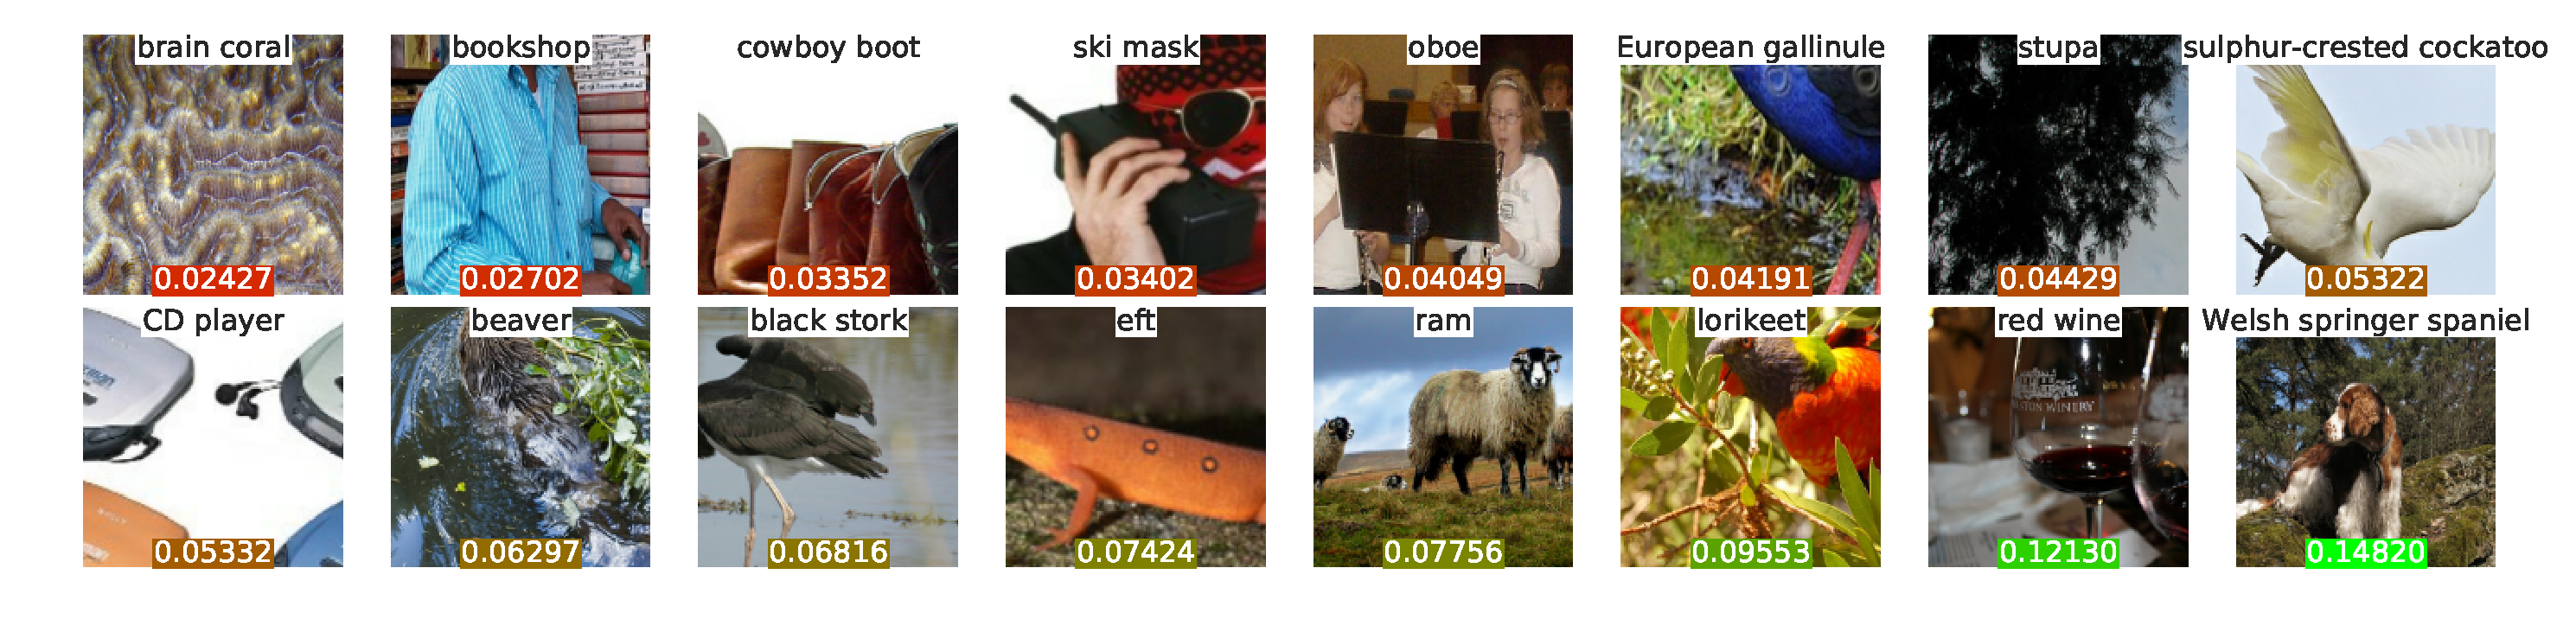
\includegraphics[width=\textwidth]{figs/imagenet_dds.eps}
    %  \vspace{-8mm}
  \caption{\label{fig:dds_score} Example images from the ImageNet and their weights assigned by \dds. A trained DDS scorer assigns higher probabilities to images from ImageNet, in which the class content is more clear. Each image's label and weight in the minibatch is shown.}
   % \vspace{-6mm}
\end{figure*}

\begin{figure}
%\begin{wrapfigure}{r}{0.3\textwidth}
  %\vspace{-12mm}
  %\begin{center}
  \centering
    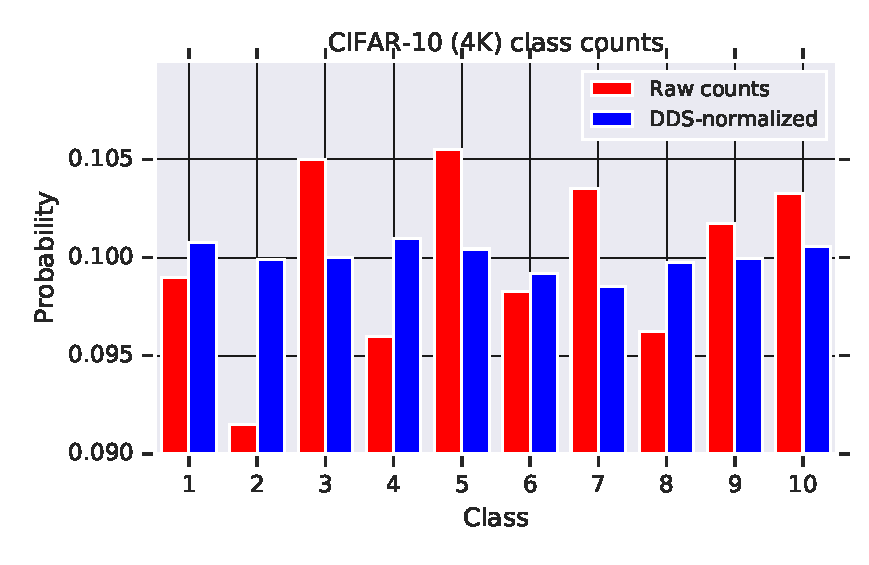
\includegraphics[width=0.4\textwidth]{figs/cifar10_dds.eps}
  %\end{center}
  %\vspace{-4mm}
  %\captionof{figure}{\label{fig:dds_distribution}Class distributions of CIFAR-10 4K.}
  \caption{\label{fig:dds_distribution}A trained DDS scorer learns to balance the class distributions of CIFAR-10 4K.}
  %\vspace{-4mm}
%\end{wrapfigure}
\end{figure}

\begin{figure}
    \centering
    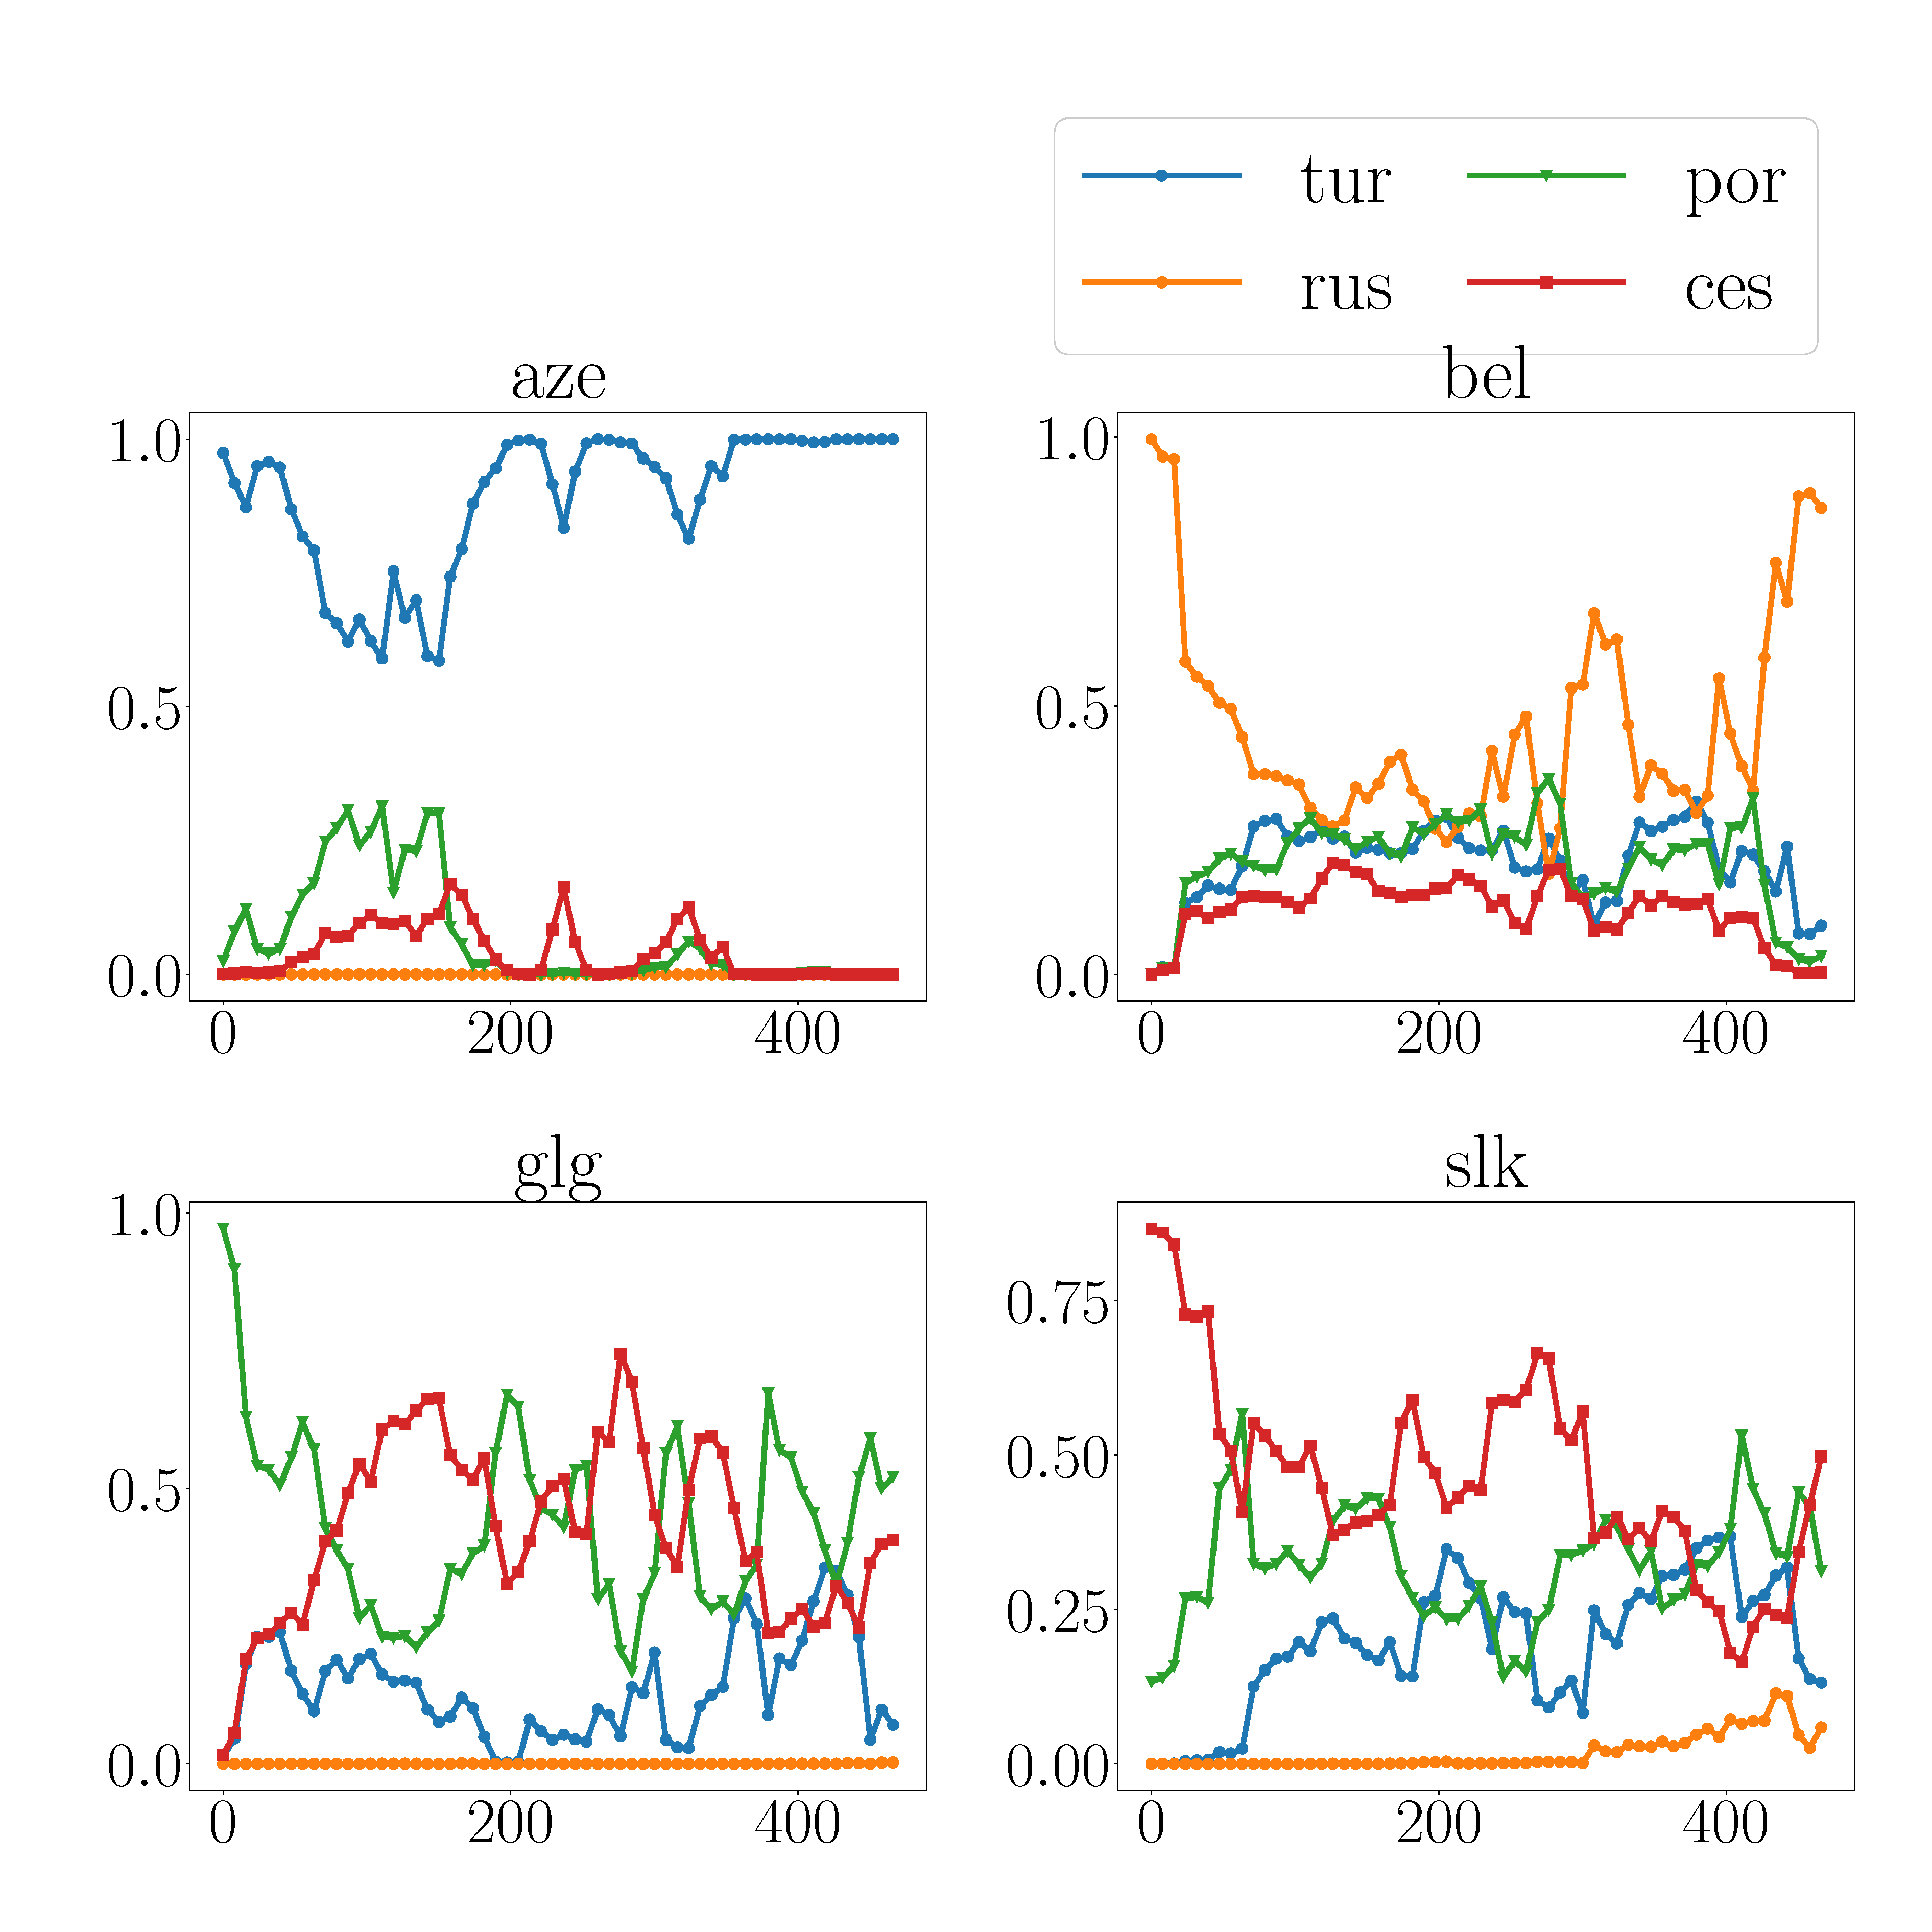
\includegraphics[width=0.9\columnwidth]{figs/hs_prob_plot.eps}
    \caption{\label{fig:nmt_distrib_hs}Language usage for TCS$+$\dds{} by training step. The distribution is initialized to focus on the most related HRL, and \dds~learns to have a more balanced usage of all languages.}
\end{figure}

\subsection{Analysis}


\textbf{Image Classification.} Prior work on heuristic data selection has found that the model performs better if we feed higher quality or more domain-relevant data  towards the end of training~\citep{dynamic_data_selection_nmt,dynamic}. Here we verify this observation by analyzing the learned importance weight at the end of training for image classification. Figure \ref{fig:dds_distribution} shows that at the end of training, \dds~learns to balance the class distribution, which is originally unbalanced due to the dataset creation. Figure \ref{fig:dds_score} shows that at the end of training, \dds~assigns higher probabilities to images with clearer class content from ImageNet. These results show that \dds~learns to focus on higher quality data towards the end of training.  


\textbf{NMT.}
Next, we focus on multilingual NMT, where the choice of data directly corresponds to picking a language, which has an intuitive interpretation. Since \dds~adapts the data weights dynamically to the model throughout training, here we analyze how the dynamics of learned weights.

%\begin{center}
%  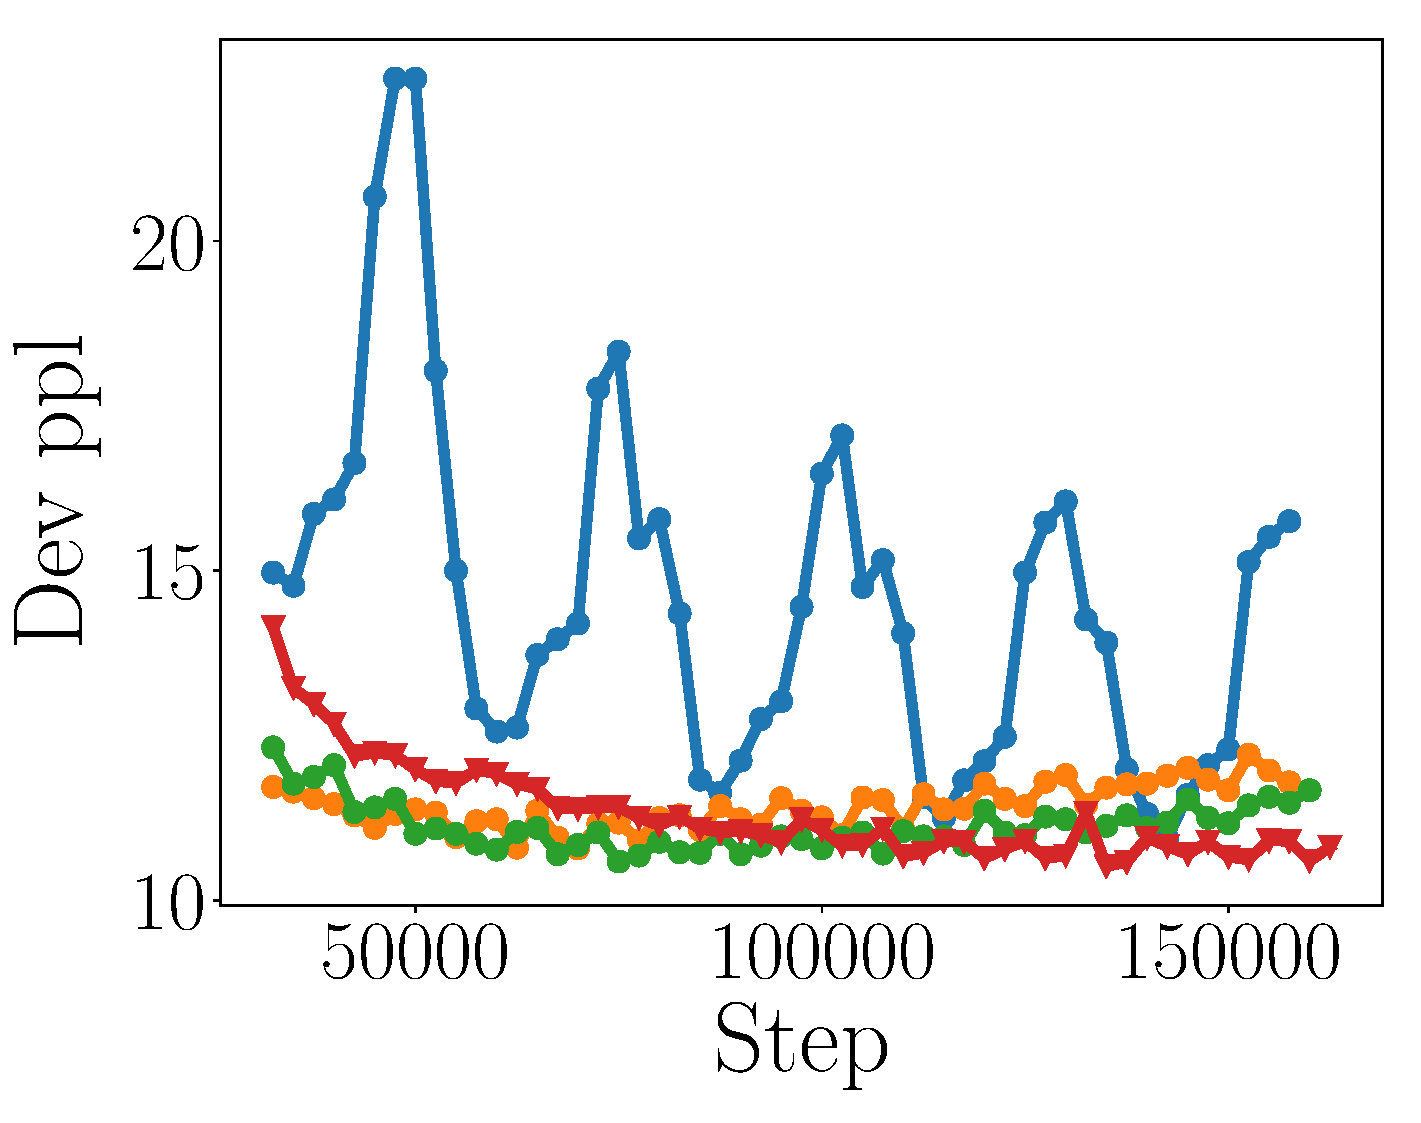
\includegraphics[width=0.245\columnwidth]{figs/aze_devppl_plot.eps}
%  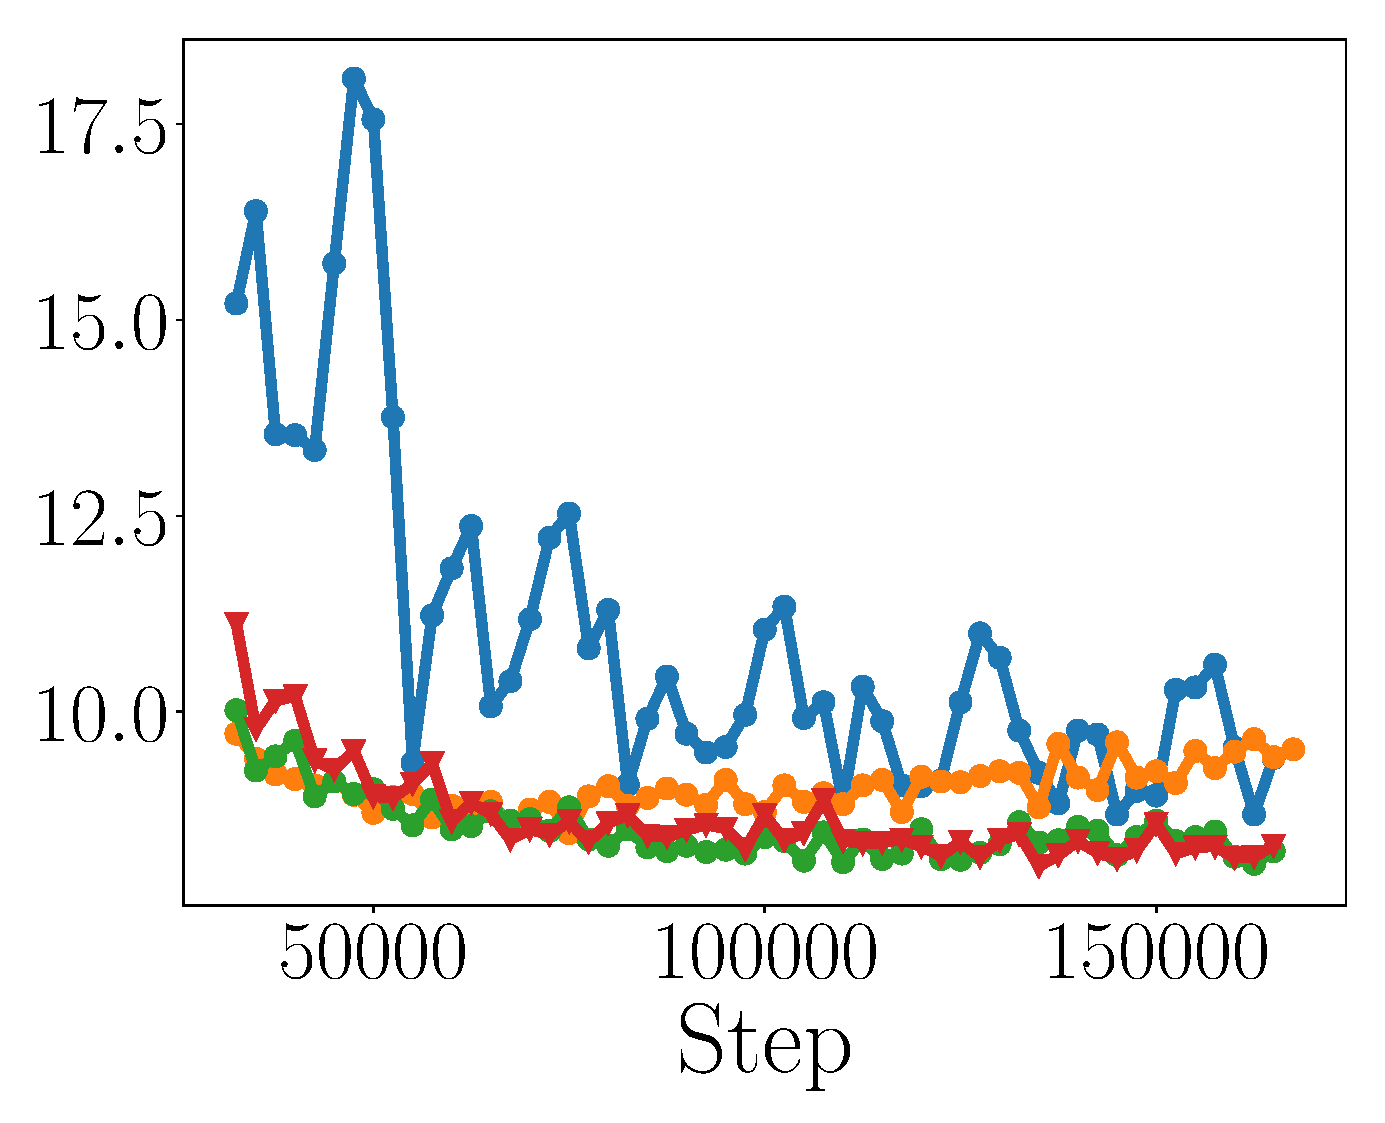
\includegraphics[width=0.23\columnwidth]{figs/bel_devppl_plot.eps}
%  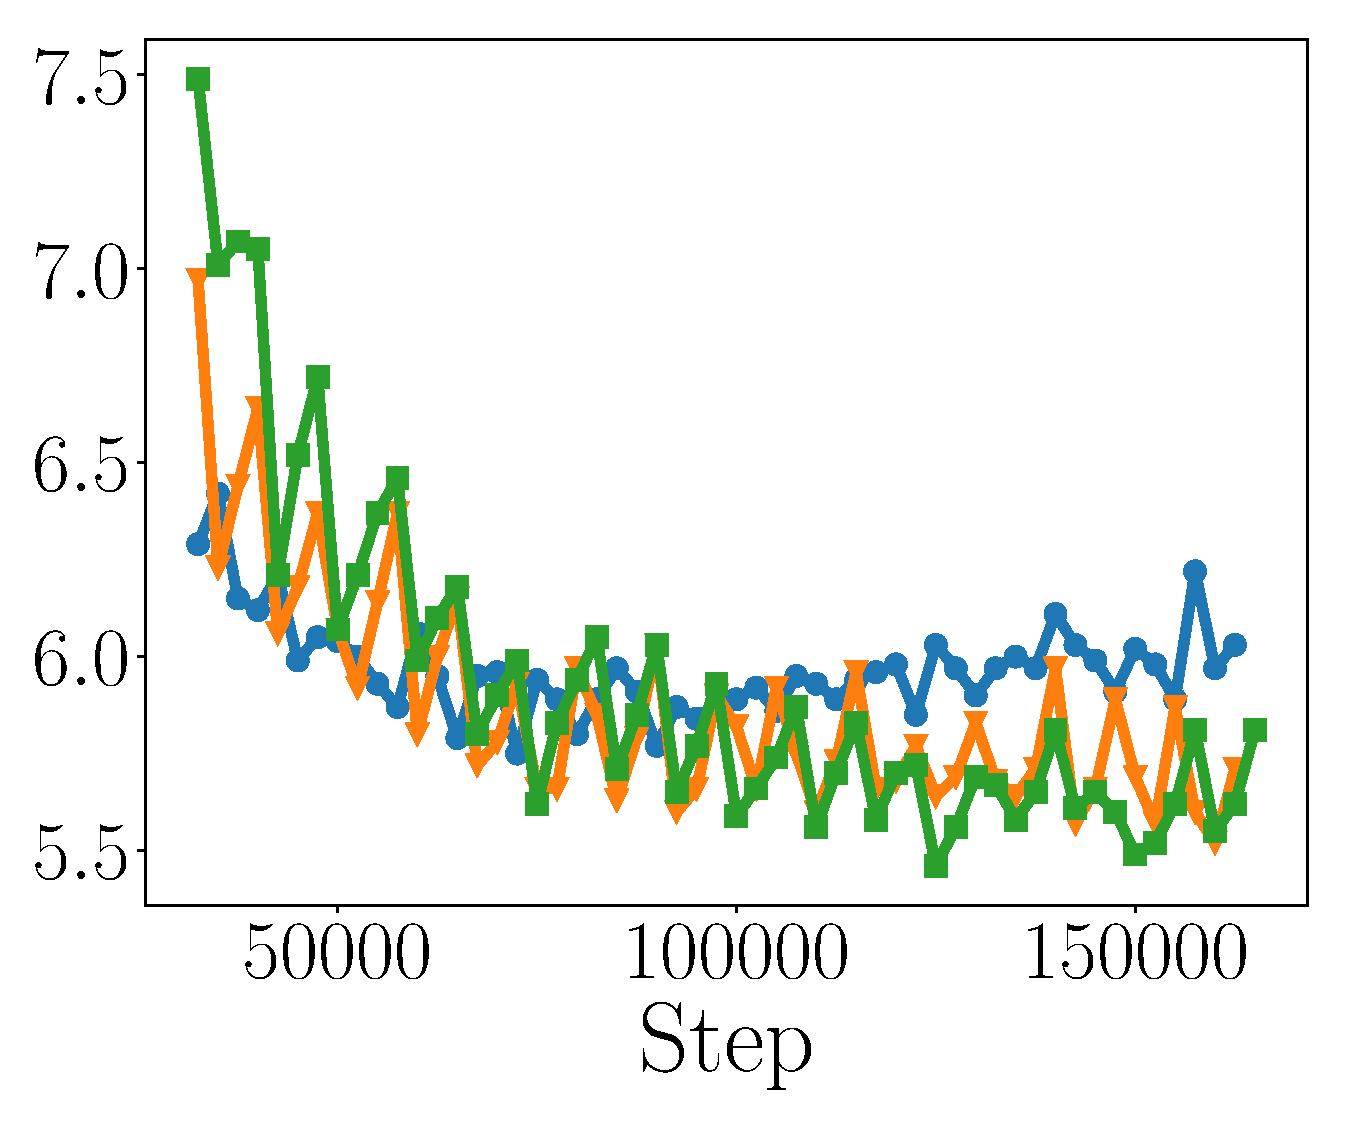
\includegraphics[width=0.23\columnwidth]{figs/glg_devppl_plot.eps}
%  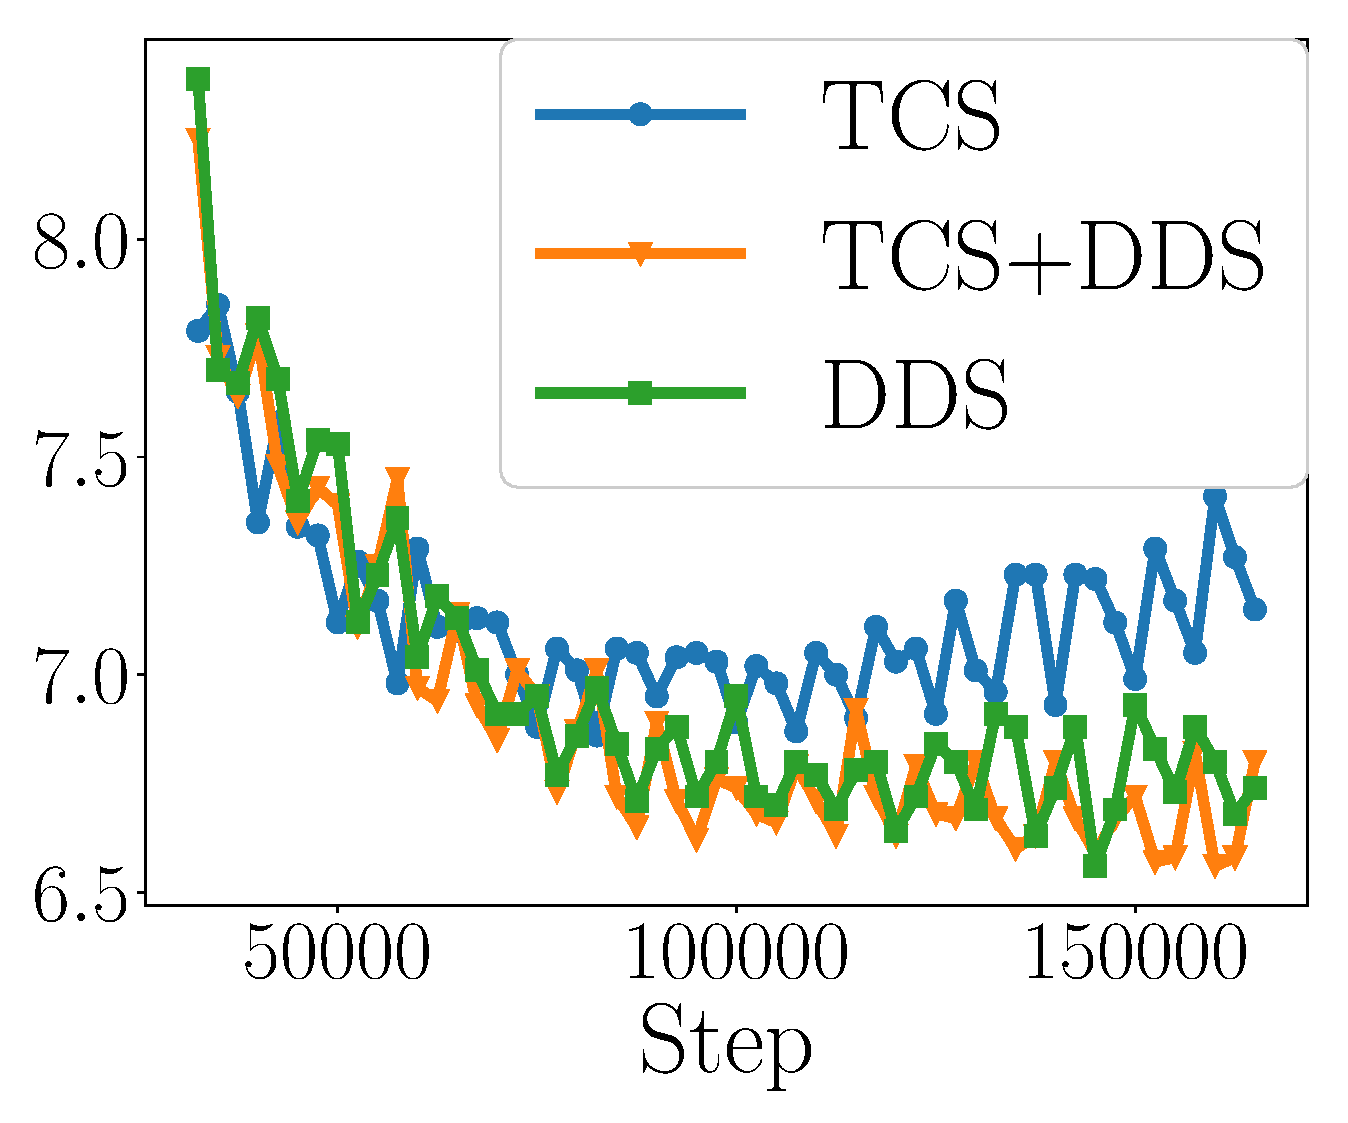
\includegraphics[width=0.23\columnwidth]{figs/slk_devppl_plot.eps}
%  \captionof{figure}{\label{fig:nmt_converge}Development set perplexity vs. training steps. \textit{From left to right}: \texttt{aze}, \texttt{bel}, \texttt{glg}, \texttt{slk}.}
%\end{center}
%\noindent \textbf{Training Curves.} First, we plot the dev set perplexity for three training methods, TCS, DDS, and TCS+DDS over the course of training in Figure \ref{fig:nmt_converge}.%
%\footnote{We did not plot ``Uniform'' here because it takes a far larger number of training steps to converge due to its uniform sampling of eight different languages, and thus is not visible on the same scale.}
%From the results, we can see that while DDS starts out with a higher perplexity than the TCS heuristics (which a-priori calculates the most appropriate language to be using based on surface statistics), it quickly catches up and surpasses TCS on all 4 languages.
%In addition, when initialized with the TCS heuristic, DDS starts at a relatively good perplexity and converges even faster.

%\begin{center}
%\centering
%  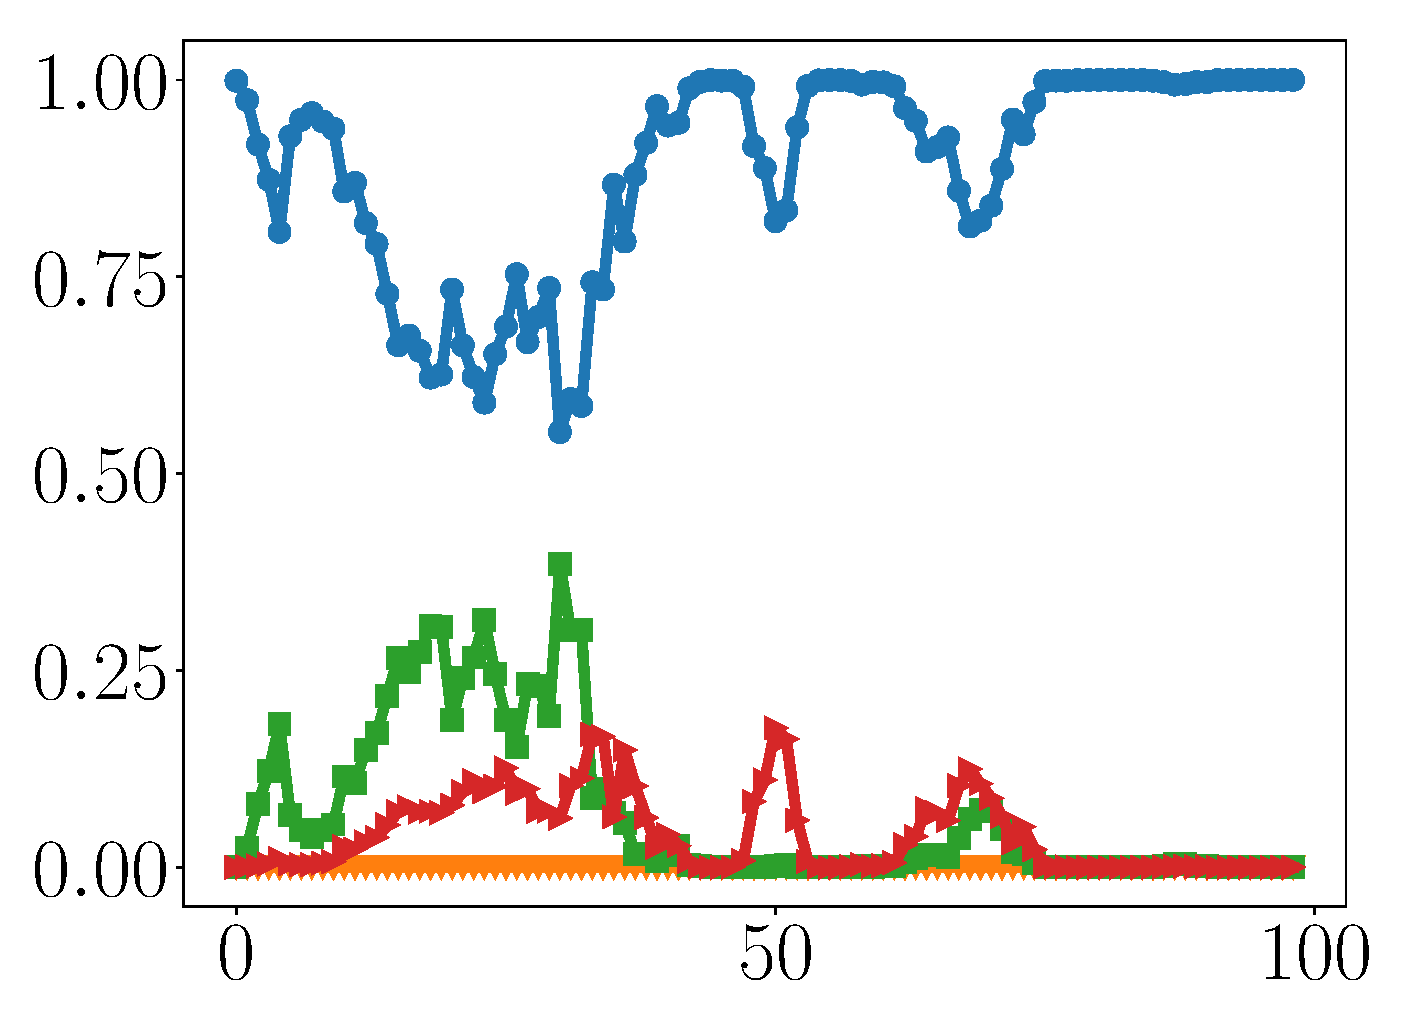
\includegraphics[width=0.4\columnwidth]{figs/aze_hs_probs_plot.eps}
%  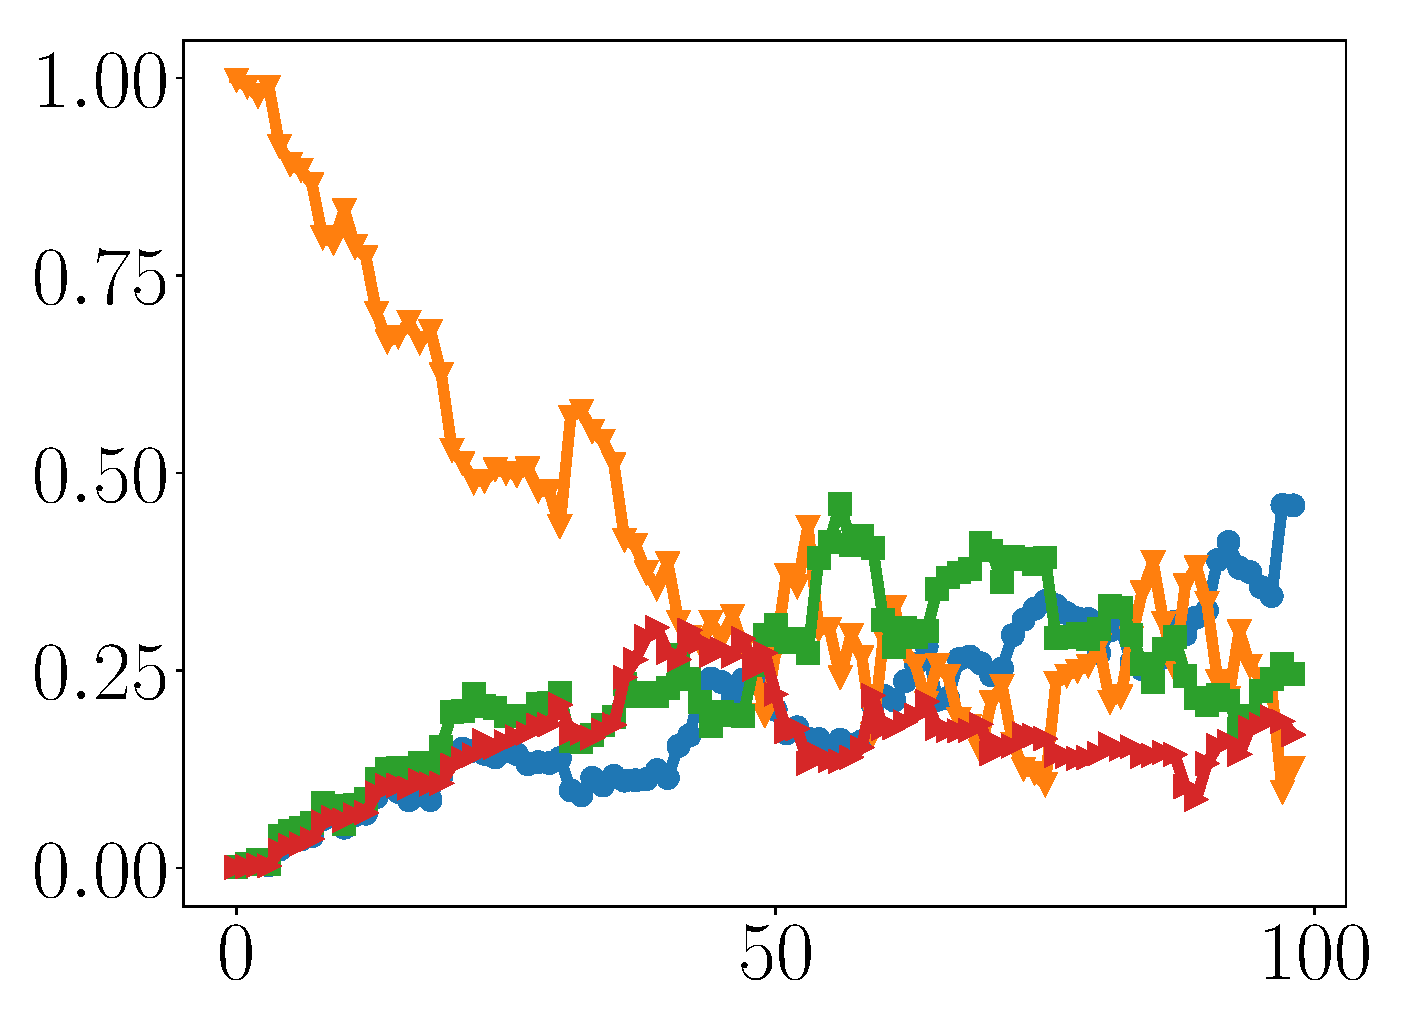
\includegraphics[width=0.4\columnwidth]{figs/bel_hs_probs_plot.eps} \quad\quad\quad\quad
%  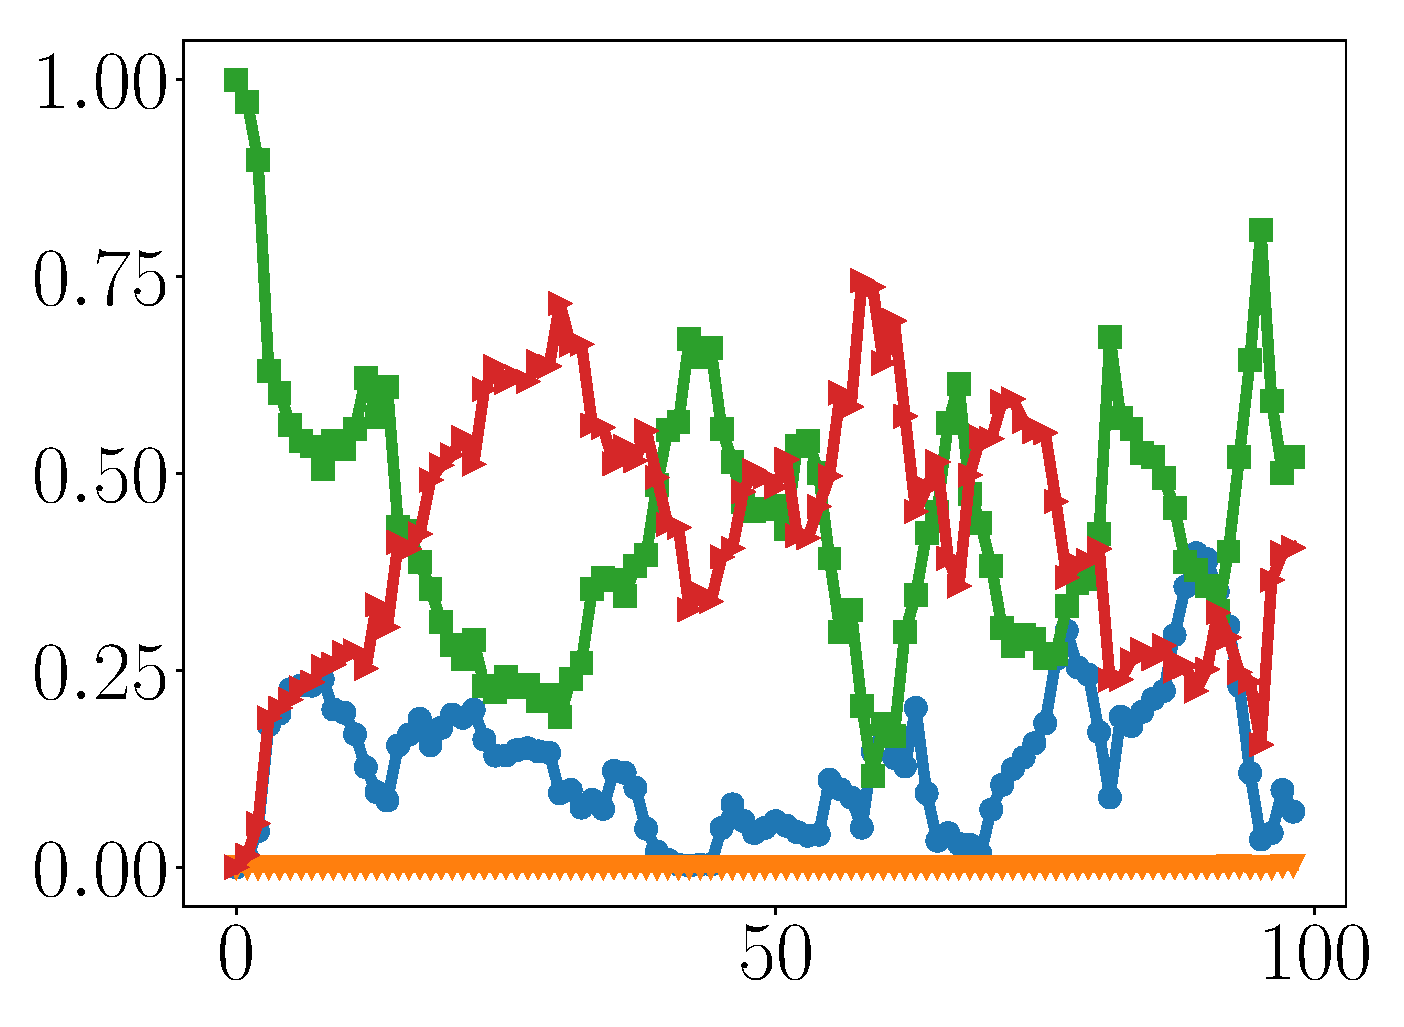
\includegraphics[width=0.4\columnwidth]{figs/glg_hs_probs_plot.eps}
%  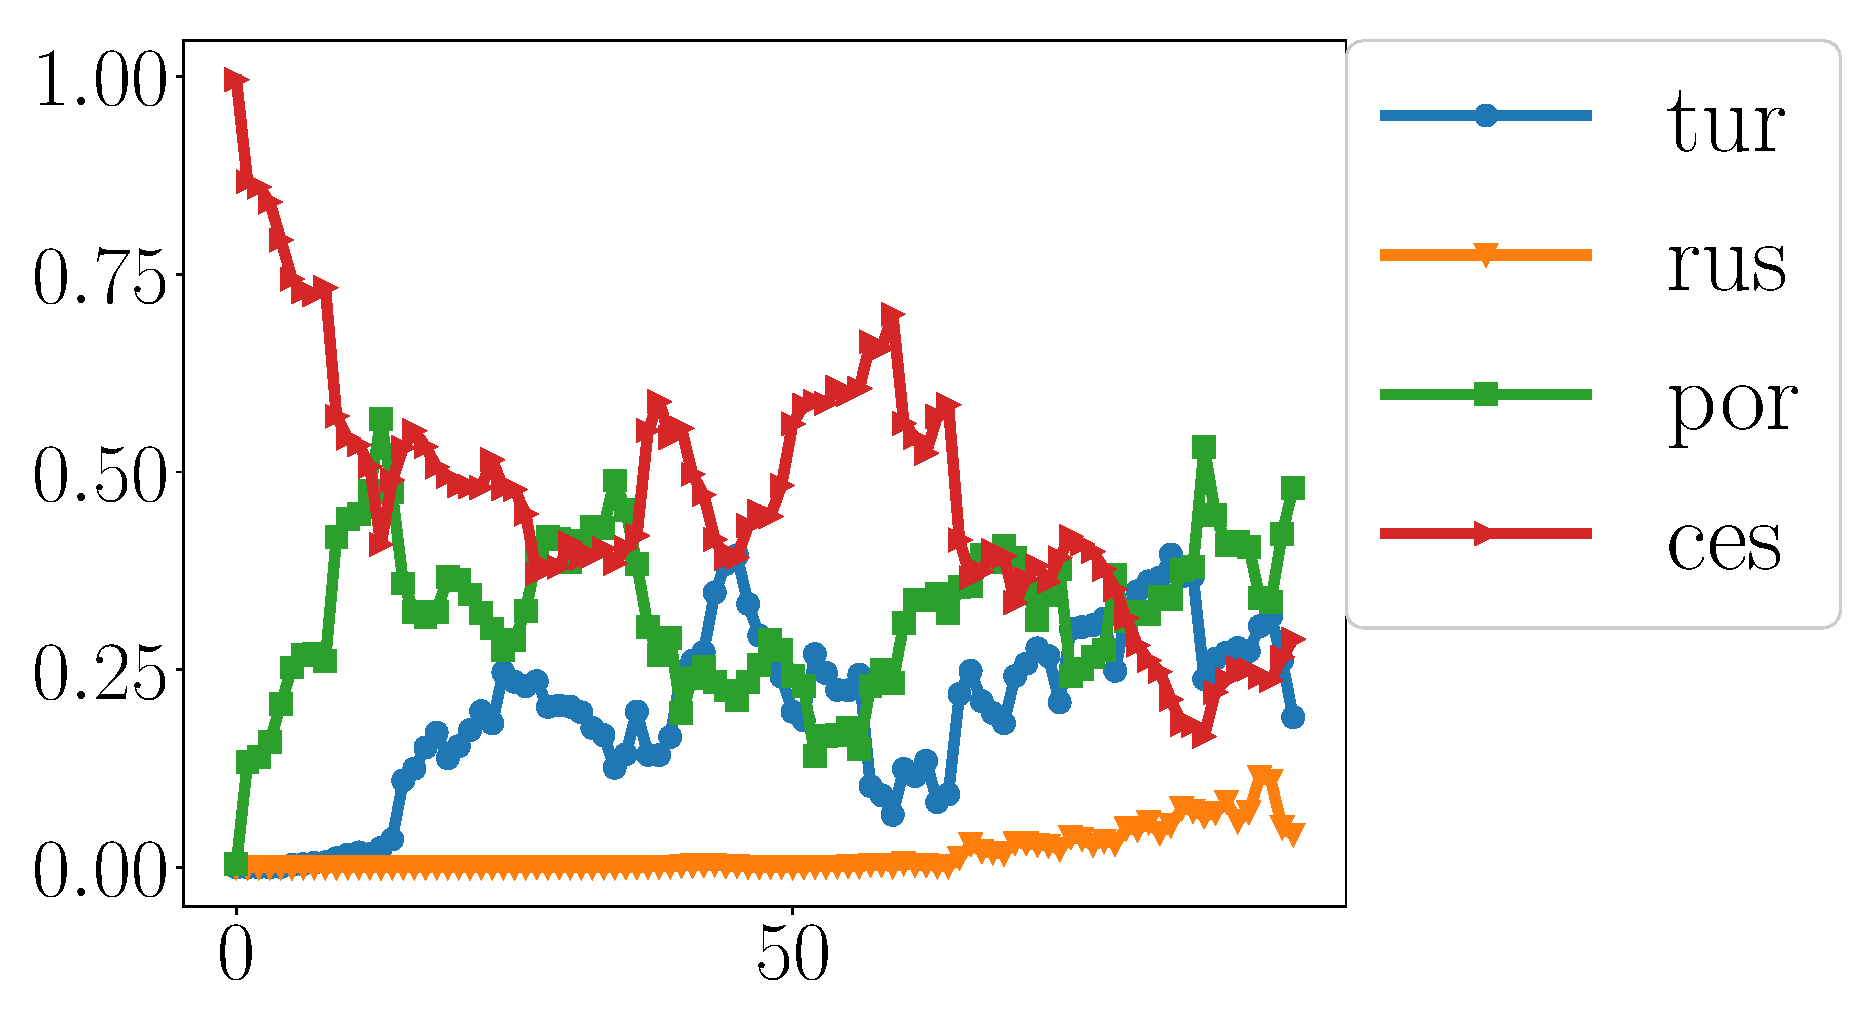
\includegraphics[width=0.5\columnwidth]{figs/slk_hs_probs_plot.eps}
%  %\captionof{figure}{\label{fig:nmt_distrib_hs}Language usage for TCS$+$\dds{} by training step. \textit{From left to right}: \texttt{aze}, \texttt{bel}, \texttt{glg}, \texttt{slk}.}
%  \caption{\label{fig:nmt_distrib_hs}Language usage for TCS$+$\dds{} by training step. \textit{From left to right}: \texttt{aze}, \texttt{bel}, \texttt{glg}, \texttt{slk}.}
%\end{center}
\begin{figure}
    \centering
    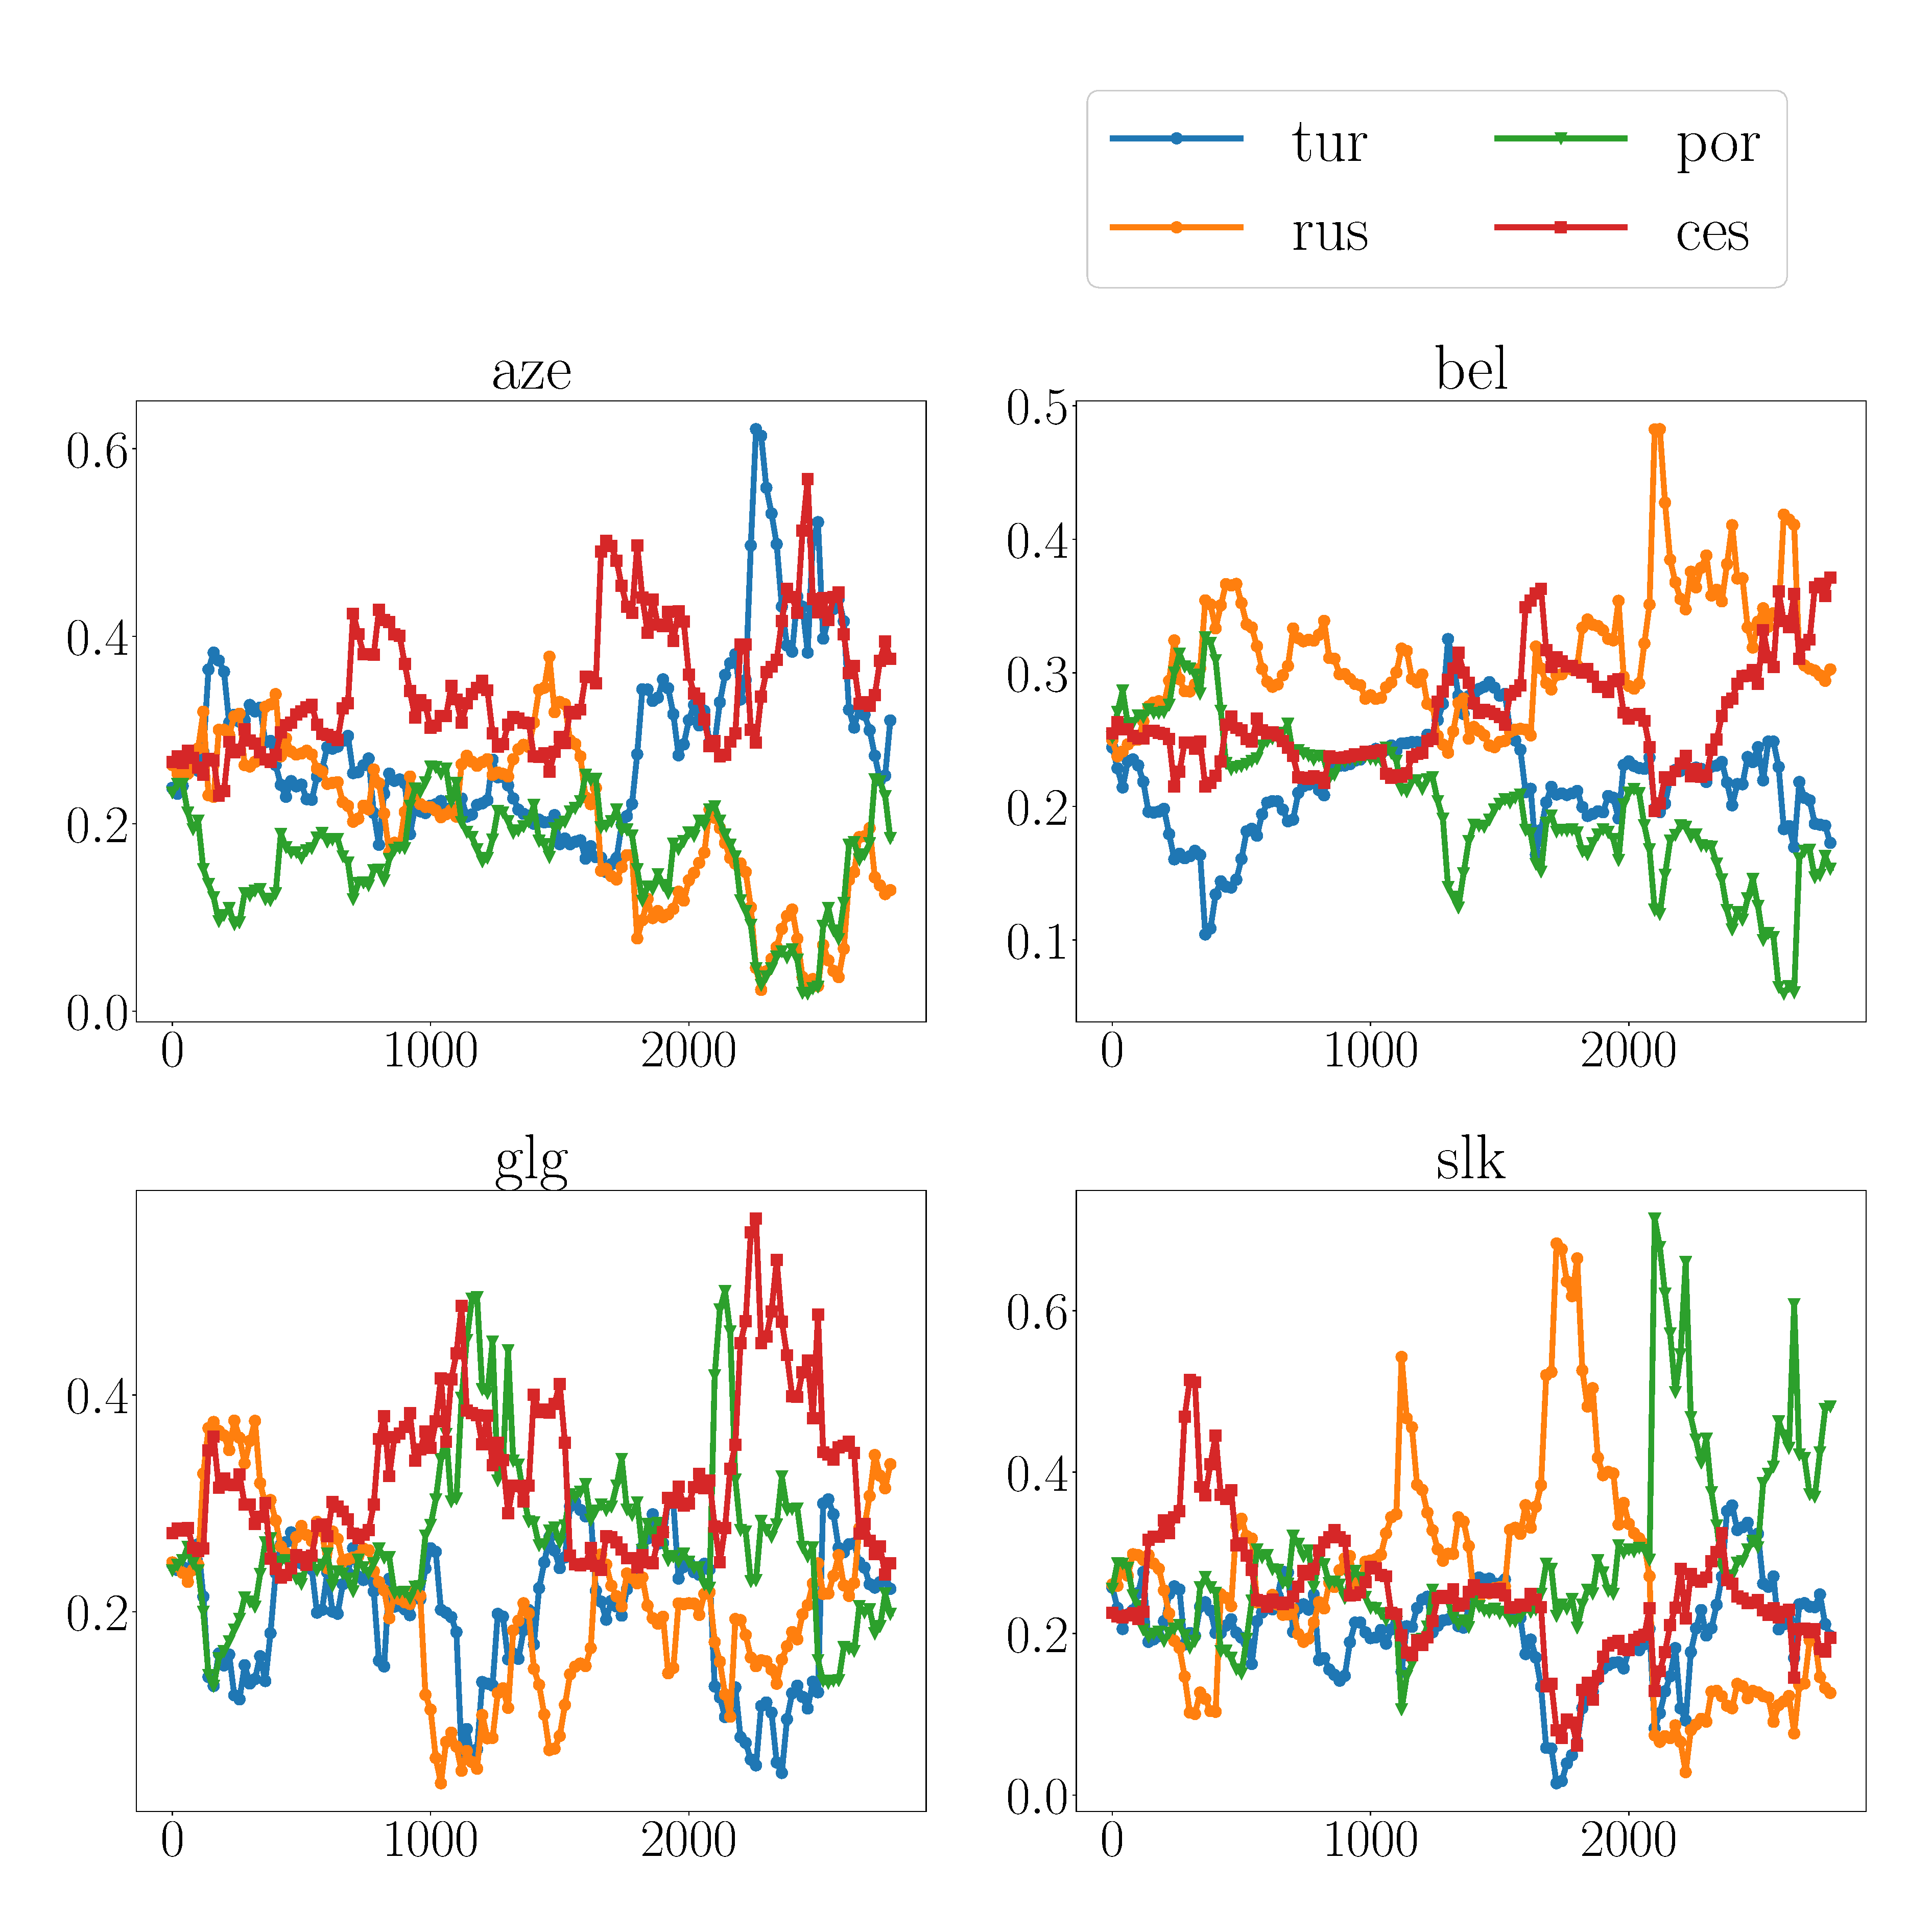
\includegraphics[width=0.9\columnwidth]{figs/uniform_prob_plot.eps}
    \caption{\label{fig:nmt_distrib_uni}Language usage for \dds~by training step. \dds~learns to upweight the most related HRL after certain training steps.}
\end{figure}
%\noindent \textbf{Learned Language Distributions.}
We plot the probability distribution of the four HRLs (because they have more data and thus larger impact on training) over the course of training.  Figure \ref{fig:nmt_distrib_hs} shows the change of language distribution for TCS+DDS. Since TCS selects the language with the largest vocabulary overlap with the LRL, the distribution is initialized to focus on the most related HRL. For all four LRLs, the percentage of their most related HRL starts to decrease as training continues. For \texttt{aze}, \dds~quickly comes back to using its most related HRL. For \texttt{gig} and \texttt{slk}, DDS learns to mainly use both \texttt{por} and \texttt{ces}, their corresponding HRL. However, for \texttt{bel}, \dds~continues the trend of using all four languages. This shows that \dds~is able to maximize the benefits of the multilingual data by having a more balanced usage of all languages. 


%For gig and slk, DDS learns to mainly use both por and ces, their corresponding HRL.

Figure \ref{fig:nmt_distrib_uni} shows a more interesting trend of \dds~without heuristic initialization.
For both \texttt{aze} and \texttt{bel}, \dds~focuses on the most related HRL after a certain number of training updates.
Interestingly, for \texttt{bel}, \dds~learns to focus on both \texttt{rus}, its most related HRL, and \texttt{ces}. Similarly for \texttt{slk}, \dds~also learns to focus on \texttt{ces}, its most related HRL, and \texttt{rus}, although there is little vocabulary overlap between \texttt{slk} and \texttt{rus}.
Also notably, the ratios change  significantly over the course of training, indicating that different types of data may be more useful during different learning stages.


%\vspace{-0.2cm}
%\begin{center}
%  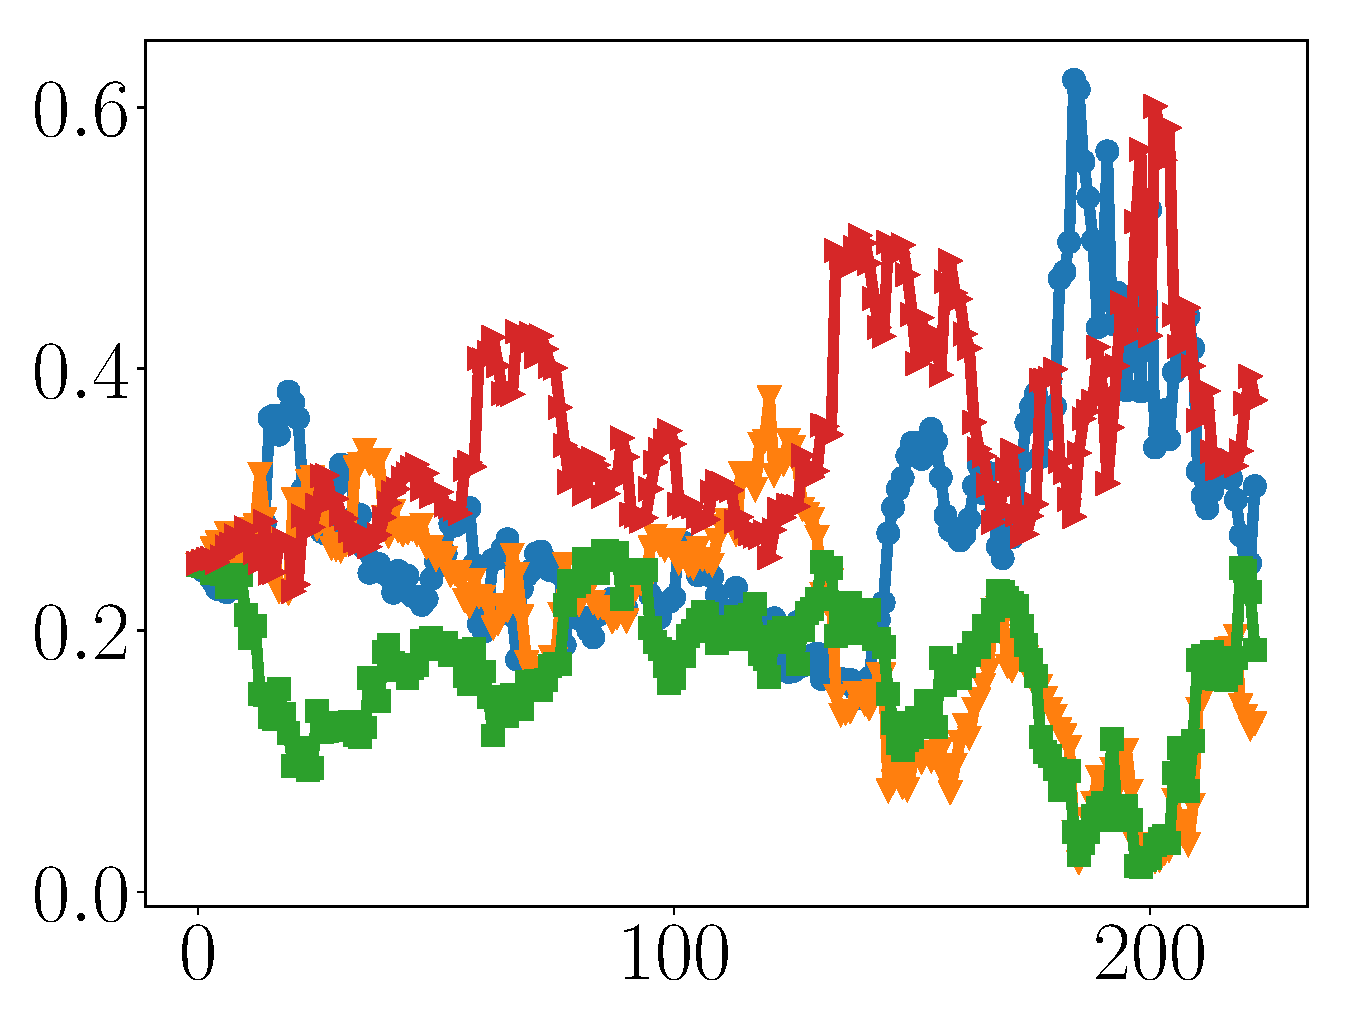
\includegraphics[width=0.20\columnwidth]{figs/aze_uni_probs_plot.eps}
%  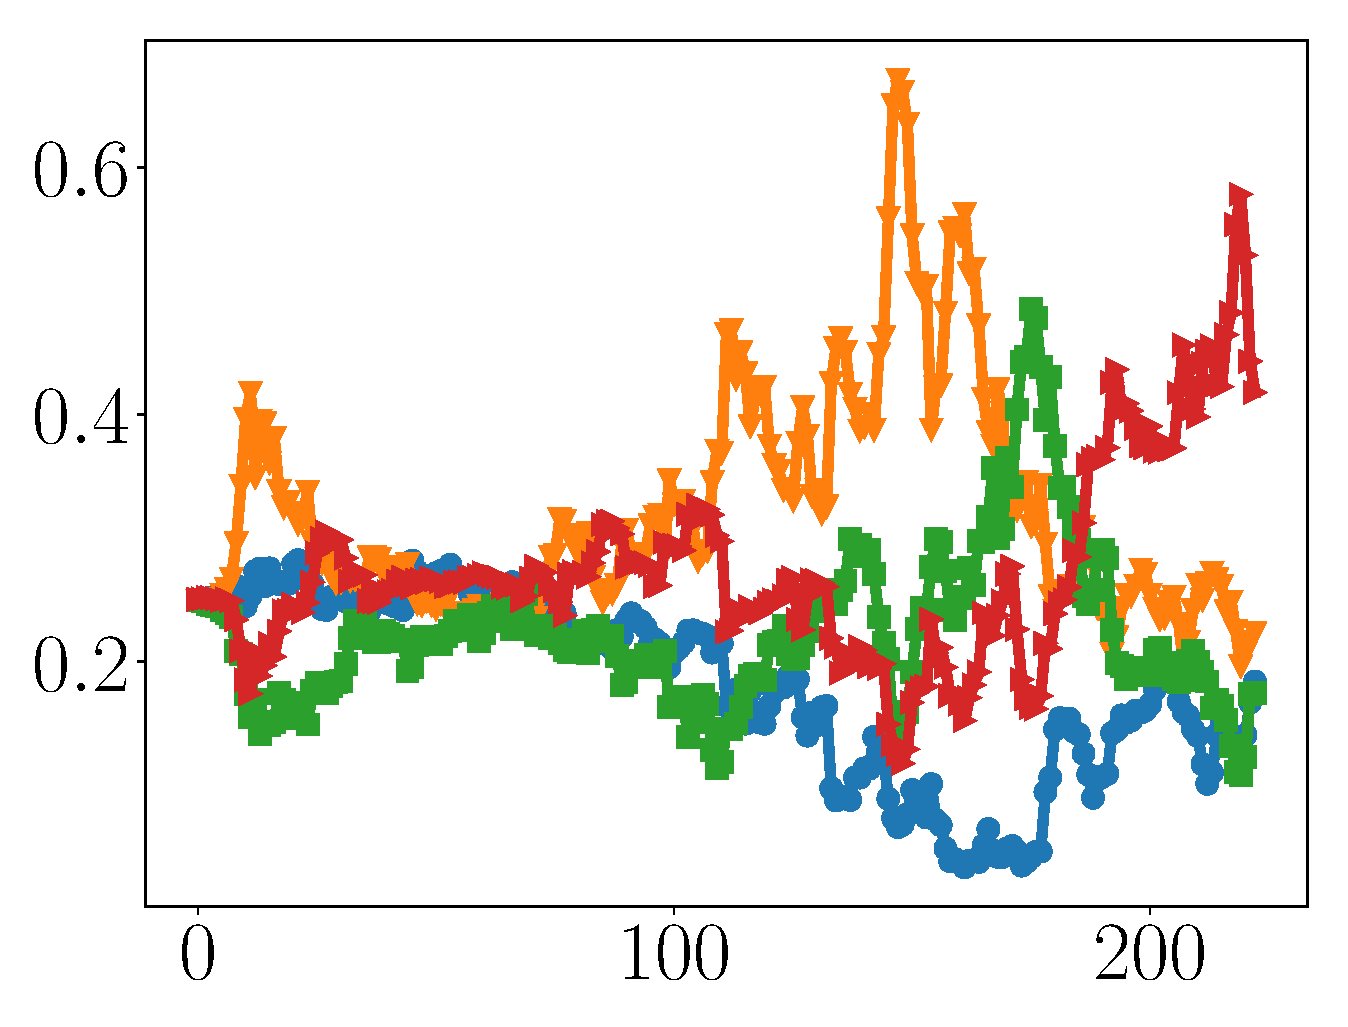
\includegraphics[width=0.20\columnwidth]{figs/bel_uni_probs_plot.eps}
%  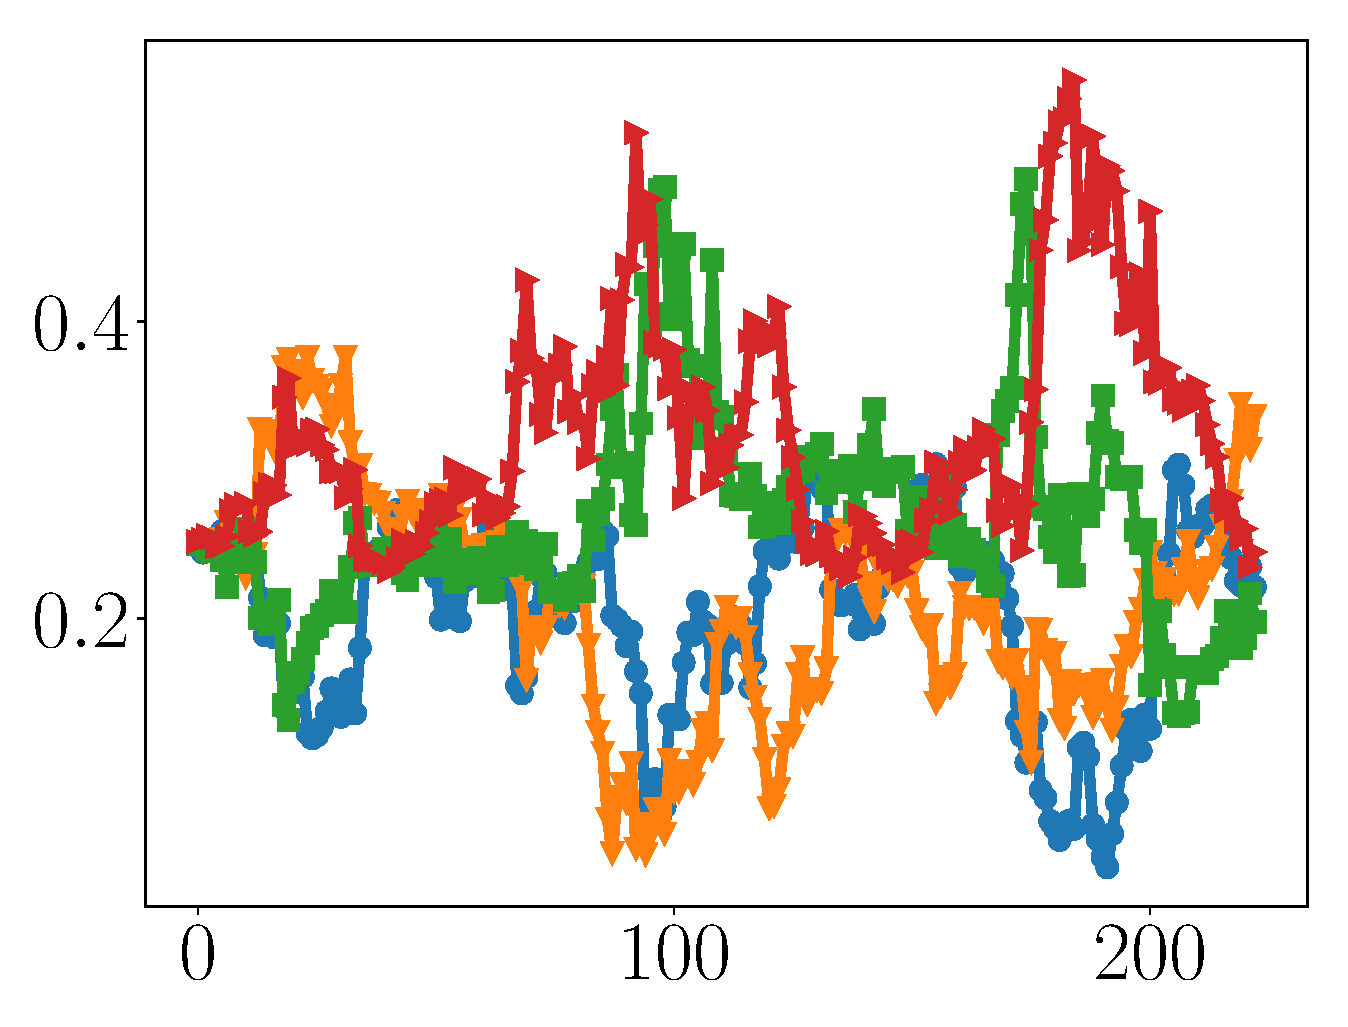
\includegraphics[width=0.2\columnwidth]{figs/glg_uni_probs_plot.eps}
%  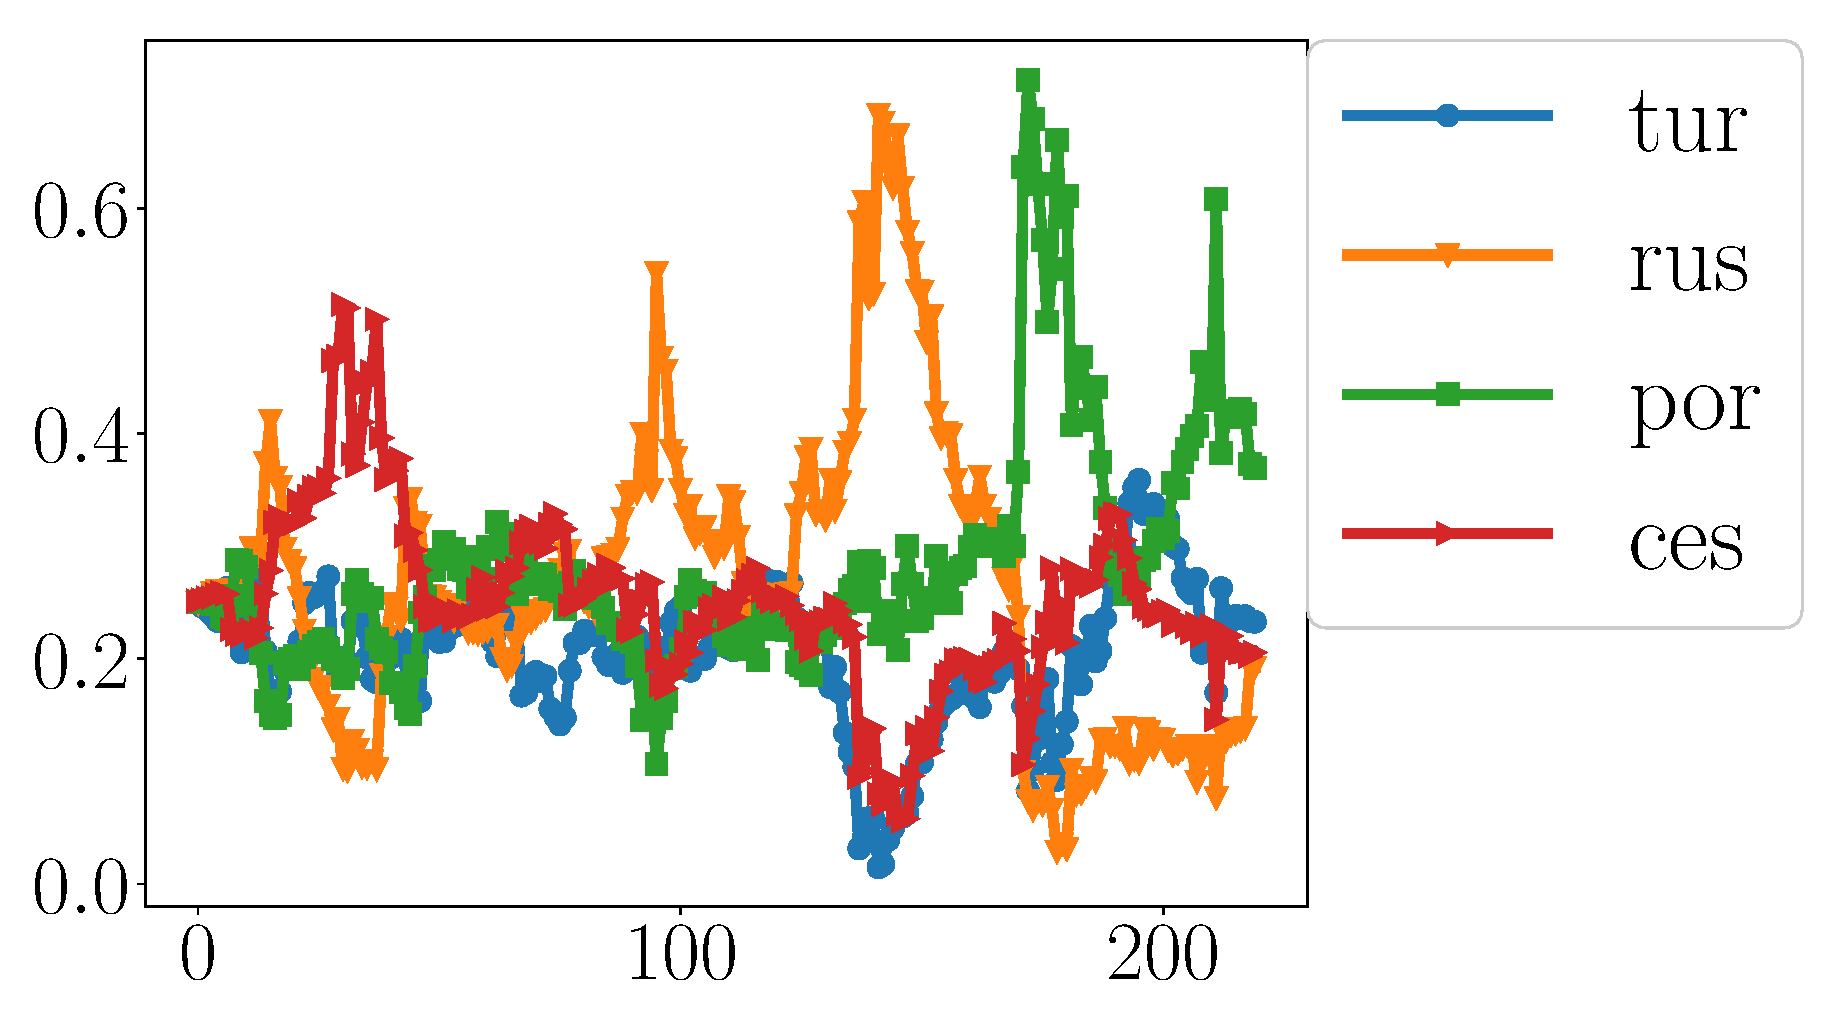
\includegraphics[width=0.25\columnwidth]{figs/slk_uni_probs_plot.eps}
%  \vspace{-0.1cm}
%  \captionof{figure}{\label{fig:nmt_distrib_uni}Language usage for \dds~by training step. \textit{From left to right}: \texttt{aze}, \texttt{bel}, \texttt{glg}, \texttt{slk}.}
%\end{center}
%\vspace{-0.1cm}


% This indicate that \dds~is able to discover the best data to use even if the patterns are not immediately intuitive.
%Similar to the trend in Figure \ref{fig:nmt_distrib_hs}, glg tends to use both por, its most related HRL, and ces. 
